\documentclass[a4paper]{article}
\usepackage{fullpage}
\oddsidemargin = -0.5in

\iffalse added for extra functionality \fi
\usepackage{booktabs}% http://ctan.org/pkg/booktabs
\newcommand{\tabitem}{~~\llap{\textbullet}~~}
\usepackage{graphicx,wrapfig,lipsum,mathtools}


\begin{document}
	\section{Opportunities}
		\subsection{What is an Opportunity?}
			According to...\\
			\begin{tabular}{ll}
				\large Schumpeter&\large Kirzner\\
				\begin{tabular}{l}
				The possibility for an opportunity comes about through\\
				macro-economic / social / political /... change.\\
				The entrepreneur uses newly available information to\\
				create an opportunity.
				\end{tabular}  & 
				\begin{tabular}{l}
				An opportunity exists because of information asymmetry \\
				in an economy.The entrepreneur could for instance \\
				be the first to see,that an item can be sold at a profit.\\ 
				Opportunities are already exist and can be discovered \\
				by the entrepreneur.
				\end{tabular}
			\end{tabular}
		\subsection{How to identify Opportunities?}
			\begin{enumerate}
				\setlength{\itemsep}{-3pt}
				\item Opportunity Analysis Canvas
				\item Business Model Canvas
				\item Business Plan
			\end{enumerate}
			
		\begin{wrapfigure}{r}{200pt}
		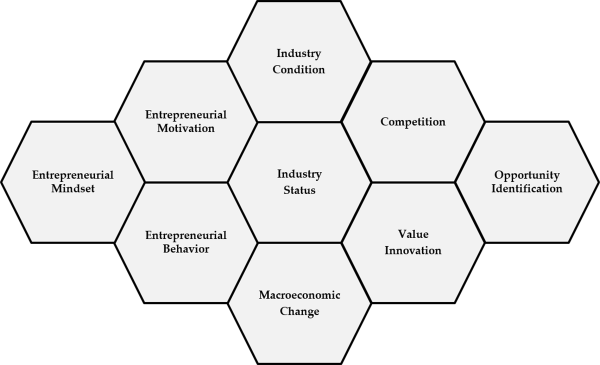
\includegraphics[width=200pt]{img/opportunityAnalysisCanvas.png}
		\end{wrapfigure}
		\subsection{Opportunity Analysis Canvas}
			The Opportunity Analysis Canvas can be split up into the parts\\
			{\bf Think, See and Act} going from left to right\\
		\subsubsection{Macro-economic changes}
			Macro-economic changes are changes like
			\begin{itemize}
			\setlength{\itemsep}{-3pt}
			{\item demographic \& social changes\\ \it{for example people becoming more health
			conscious}}
			{\item technological changes\\ {\it for example smartphones}}
			{\item political \& regulatory changes\\ \it{for example ACTA}}
			\end{itemize}
			All these changes bring opportunities
		\subsubsection{Competition}
			You have to assess your competition by looking at their and your
			\begin{enumerate}
			\setlength{\itemsep}{-3pt}
			\item learning curve
				\begin{itemize}
				\setlength{\itemsep}{-3pt}
				\item how long will it take for you to catch up to each other
				\item how fast can you each react to new markets/products
				\end{itemize}
			\item complementary assets
				\begin{itemize}
				\setlength{\itemsep}{-3pt}
				\item money, knowledge and relationships to share
				\item how can you feed of each others reputation (reputation effect)
				\end{itemize}
			\end{enumerate}
		\subsubsection{Industry condition}
			\begin{itemize}
			\setlength{\itemsep}{-3pt}
			\item how much knowledge is required in the industry?
			\item how much demand is there?
			\item is the industry growing?
			\item is the industry focused on capital and/or advertising?
			\item in what stage of development is the industry? (industry life cycle)
			\end{itemize}
	\section{Entrepreneurship}
		\begin{tabular}{ll}
			\large Why?&\large Why not?\\
			\tabitem money & \tabitem risk\\
			\tabitem independence & \tabitem failure\\
			\tabitem freedom & \tabitem pressure\\
			\tabitem creating something & \\
			\tabitem helping others & \\
		\end{tabular}
	\section{Pattern of development and diffusion}
		{\LARGE We have an {\bf Invention} $\xrightarrow[]{}$ What now?}\\\\
		\begin{tabular}{ll}
			{\bf\large Model1}&{\bf\large Model2}\\\\
			\begin{minipage}[t]{0.4\textwidth}
				{\bf Life Cycle Model}
				\begin{itemize}
				\setlength{\itemsep}{-3pt}
				\item develop product out of invention
				\item after introduction people slowly adapt
				\item the initial boom eventually slows down
				\item boom happens in s-curve pattern which is called "pattern of diffusion"
				\item innovation is seen as a managing competence
				\end{itemize}
			\end{minipage}
			&
			\begin{minipage}[t]{0.4\textwidth}
				{\bf Evolution Model}
				\begin{itemize}
				\setlength{\itemsep}{-3pt}
				\item after the invention it takes on average {\bf a decade} until the product is 
				released
				\item it takes many trial and error attempts before the final product
				\item the Life Cycle Model comes in once the product is succesfully released
				\item innovation is seen as proces of trial and error
				\end{itemize}
			\end{minipage}
		\end{tabular}\\\\
		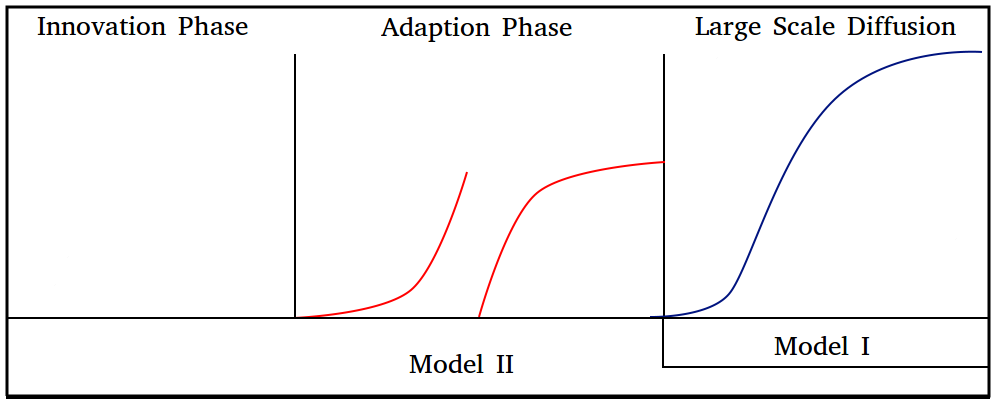
\includegraphics[width=400pt]{img/patternOfDiffusionModel.png}\\
		Special points:
		\begin{itemize}
		\item Model1 is a special case of Model2 (20\% of cases are Model1) 
		\item Model1 works if there {\bf is already a market} for the product and the {\bf problem for 
		the product to solve is known}
		\end{itemize}
		\begin{tabular}{ll}
			\begin{minipage}[t]{0.4\textwidth}
				{\bf Life Cycle Model}
				\begin{itemize}
				\setlength{\itemsep}{-3pt}
				\item success == defusion
				\item success is predictable
				\item new technology is better than old technology
				\item innovation can be seen as a project
				\end{itemize}
			\end{minipage}
			&
			\begin{minipage}[t]{0.4\textwidth}
				{\bf Evolution Model}
				\begin{itemize}
				\setlength{\itemsep}{-3pt}
				\item success comes through well timed and entrepreneurial action
				\item innovation cannot be seen as a project (it is not plannable)
				\end{itemize}
			\end{minipage}
		\end{tabular}
\end{document}